\documentclass[11pt,compress,t,notes=noshow]{beamer}\usepackage[]{graphicx}\usepackage[]{color}

\makeatletter
\def\maxwidth{ %
  \ifdim\Gin@nat@width>\linewidth
    \linewidth
  \else
    \Gin@nat@width
  \fi
}
\makeatother

\definecolor{fgcolor}{rgb}{0.345, 0.345, 0.345}
\newcommand{\hlnum}[1]{\textcolor[rgb]{0.686,0.059,0.569}{#1}}%
\newcommand{\hlstr}[1]{\textcolor[rgb]{0.192,0.494,0.8}{#1}}%
\newcommand{\hlcom}[1]{\textcolor[rgb]{0.678,0.584,0.686}{\textit{#1}}}%
\newcommand{\hlopt}[1]{\textcolor[rgb]{0,0,0}{#1}}%
\newcommand{\hlstd}[1]{\textcolor[rgb]{0.345,0.345,0.345}{#1}}%
\newcommand{\hlkwa}[1]{\textcolor[rgb]{0.161,0.373,0.58}{\textbf{#1}}}%
\newcommand{\hlkwb}[1]{\textcolor[rgb]{0.69,0.353,0.396}{#1}}%
\newcommand{\hlkwc}[1]{\textcolor[rgb]{0.333,0.667,0.333}{#1}}%
\newcommand{\hlkwd}[1]{\textcolor[rgb]{0.737,0.353,0.396}{\textbf{#1}}}%
\let\hlipl\hlkwb

\usepackage{framed}
\makeatletter
\newenvironment{kframe}{%
 \def\at@end@of@kframe{}%
 \ifinner\ifhmode%
  \def\at@end@of@kframe{\end{minipage}}%
  \begin{minipage}{\columnwidth}%
 \fi\fi%
 \def\FrameCommand##1{\hskip\@totalleftmargin \hskip-\fboxsep
 \colorbox{shadecolor}{##1}\hskip-\fboxsep
     \hskip-\linewidth \hskip-\@totalleftmargin \hskip\columnwidth}%
 \MakeFramed {\advance\hsize-\width
   \@totalleftmargin\z@ \linewidth\hsize
   \@setminipage}}%
 {\par\unskip\endMakeFramed%
 \at@end@of@kframe}
\makeatother

\definecolor{shadecolor}{rgb}{.97, .97, .97}
\definecolor{messagecolor}{rgb}{0, 0, 0}
\definecolor{warningcolor}{rgb}{1, 0, 1}
\definecolor{errorcolor}{rgb}{1, 0, 0}
\definecolor{code}{rgb}{0.97, 0.96, 1.0}
\newenvironment{knitrout}{}{} % an empty environment to be redefined in TeX

\usepackage{alltt}
\usepackage[utf8]{inputenc}
\usepackage[ngerman]{babel}
\usepackage{dsfont}
\usepackage{verbatim}
\usepackage{amsmath}
\usepackage{amsfonts}
\usepackage{mathtools}
\usepackage{csquotes}
\usepackage{cmbright}
\usepackage{multirow}
\usepackage{longtable}
\usepackage{enumerate}
\usepackage[absolute,overlay]{textpos}
\usepackage{psfrag}
\usepackage{algorithm}
\usepackage{algpseudocode}
\usepackage{eqnarray}
\usepackage{bytefield}
\usepackage{animate}
\usepackage{tikz}
\usetikzlibrary{shapes,matrix,positioning,chains,arrows,shadows,decorations.pathmorphing,fit,backgrounds}
\usepackage{adjustbox}
\usepackage{colortbl}
\usepackage{tabularx} % for tables (incl. \hline)
\usepackage{arydshln} % Load after array, longtable, colortab and/or colortbl , otherwise problems with \hline in tabular env
\usepackage{etex} %increase registers for \dimenS to more than 256, otherwise we get "No room for a new \dimen"
\usepackage{graphicx}
\usepackage{booktabs} %used in epr lectures
\usepackage{bm} % bold greek letters
\usepackage{hyperref} % url citing
\usepackage{blkarray} % block arrays
\usepackage{listings} % block of code
\usepackage{xcolor} %colored math symbols
\usepackage{pgffor}
\usepackage{verbatimbox}
\usepackage{xcolor}

%some colors
\definecolor{checkgreen}{HTML}{18A126}
\definecolor{errorred}{HTML}{FF0000}
\definecolor{blockbg}{HTML}{F7F7F7}
\definecolor{gray}{HTML}{A0A0A0}

% basic latex stuff
\newcommand{\col}{\par\colorbox{code}{\parbox{\textwidth}{\theverbbox}}\par}
\newcommand{\eg}{e.\,g.\xspace} %for example
\newcommand{\ie}{i.\,e.\xspace} %that is to say...
\newcommand{\pkg}[1]{{\fontseries{b}\selectfont #1}} %fontstyle for R packages
\newcommand{\lz}{\vspace{0.5cm}} %vertical space
\newcommand{\oneliner}[1] % Oneliner for important statements
{\begin{block}{}\begin{center}\begin{Large}#1\end{Large}\end{center}\end{block}}
\def\SpAr{\quad \Rightarrow \quad}

%new environments
\newenvironment{vbframe}  %frame with breaks and verbatim
{
 \begin{frame}[containsverbatim,allowframebreaks]
}
{
\end{frame}
}

\newenvironment{vframe}  %frame with verbatim without breaks (to avoid numbering one slided frames)
{
 \begin{frame}[containsverbatim]
}
{
\end{frame}
}

\newenvironment{blocki}[1]   % itemize block
{
 \begin{block}{#1}\begin{itemize}
}
{
\end{itemize}\end{block}
}

\newenvironment{fragileframe}[2]{  %fragile frame with framebreaks
\begin{frame}[allowframebreaks, fragile, environment = fragileframe]
\frametitle{#1}
#2}
{\end{frame}}

\newcommand{\myframe}[2]{  %short for frame with framebreaks
\begin{frame}[allowframebreaks]
\frametitle{#1}
#2
\end{frame}}

\usepackage{../../style/lmu-lecture}

\let\code=\texttt
\let\proglang=\textsf

\setkeys{Gin}{width=0.9\textwidth}

\usepackage{tikz}
\usetikzlibrary{shapes,arrows,snakes, calc}

% Define block styles
\tikzstyle{decision} = [diamond, draw, text width=6em, text badly centered, node distance=4cm, inner sep=0pt]
\tikzstyle{decision2} = [diamond, draw, fill=customgreen!35, text width=6em, text badly centered, node distance=4cm, inner sep=0pt]

\tikzstyle{block} = [rectangle, draw, text width=14em, text centered, rounded corners, node distance=3cm, minimum height=4em]
\tikzstyle{line} = [draw, -latex']
\tikzstyle{cloud} = [draw, ellipse, node distance=3cm, minimum height=2em]

\title{Introduction to Deep Learning}
\author{Bernd Bischl}
\institute{Department of Statistics -- LMU Munich}
\date{WS 2021/2022}

\setbeamertemplate{frametitle}{\expandafter\uppercase\expandafter\insertframetitle}

\IfFileExists{upquote.sty}{\usepackage{upquote}}{}
\input{../../latex-math/basic-math}
\input{../../latex-math/basic-ml}
\input{../../latex-math/ml-nn}

\begin{document}

\lecturechapter{2}{Single Neuron / Preceptron}
\lecture{I2DL}
%%%%%%%%%%%%%%%%%%%%%%%%%%%%%%%%%%%%%%%%%%%%%%%%%%%%%%%%%%%%%%%%%%

\begin{frame} {A Single Neuron}
\begin{itemize}
\item To illustrate the types of functions that neural networks can represent, let us begin with a simple model: logistic regression.
\vspace{5mm}
\item The hypothesis space of logistic regression can be written as follows, where $\tau(z) = (1 + \exp(-z))^{-1}$ is the logistic sigmoid function:
\begin{small} 
$$\Hspace = \left\{f: \R^p \to [0, 1] ~\bigg|~ \fx = \tau\left(\sum_{j = 1}^p w_j x_j + b\right), \wtw \in \R^p, b \in \R \right\},$$ \end{small}
\vspace{3mm}
\item It is straightforward to represent $\fx$ graphically as a neuron.
\vspace{5mm}
\item Note: $\wtw$ and $b$ together constitute $\thetab$.
\end{itemize}
\end{frame}
%%%%%%%%%%%%%%%%%%%%%%%%%%%%%%%%%%%%%%%%%%%%%%%%%%%%%%%%%%%%%%%%%%

\begin{vbframe} {A Single Neuron}
\begin{figure}
\centering
\scalebox{.4}{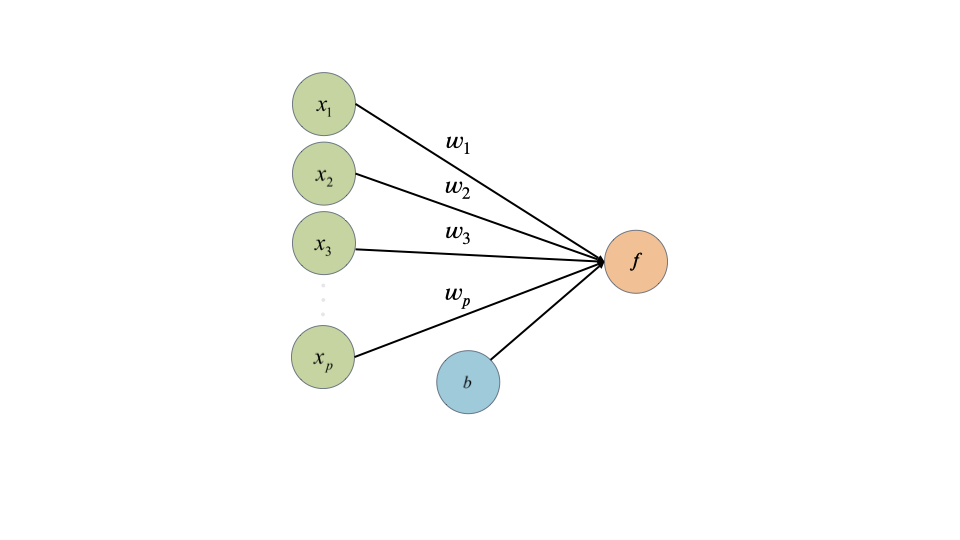
\includegraphics{figure/perceptron_tau.png}}
\end{figure}
\vspace{-2mm}
\footnotesize Perceptron $z$, with \textbf{input features} $x_1, x_2, ... ,x_p$, \textbf{weights} $w_1, w_2,... ,w_p$, \textbf{bias term} $b$ and \textbf{activation function} $\tau$.
\vspace{.2cm}
\normalsize
\begin{itemize}
\item The perceptron is the basic computational unit for neural networks.
\vspace{.2cm}
\item It is a weighted sum of input values, transformed by $\tau$:
\vspace{-1mm}
$$y = \tau(w_1x_1 + ... + w_px_p +  b) = \tau(w^T x+b)$$
\end{itemize}
\end{vbframe}
%%%%%%%%%%%%%%%%%%%%%%%%%%%%%%%%%%%%%%%%%%%%%%%%%%%%%%%%%%%%%%%%%%

\begin{vbframe}{A Single Neuron}
\textbf{Choices for $\tau$:} a single neuron can represent different functions if we choose a suitable activation function for it.
\vspace{.5cm}
\begin{itemize}
\item The identity function gives us the simple \textbf{linear regression}:
$$y = \tau(w^T x) = w^T x$$
\vspace{.5cm}
\item The logistic function gives us the \textbf{logistic regression}:
$$y = \tau(w^T x) = \frac{1}{1 + \exp(-w^T x)}$$
\end{itemize}
\end{vbframe}
%%%%%%%%%%%%%%%%%%%%%%%%%%%%%%%%%%%%%%%%%%%%%%%%%%%%%%%%%%%%%%%%%%

\begin{vbframe} {A Single Neuron}
We consider a logistic regression model for $p = 3$, i.e. $\fx = \tau(w_1\textcolor{red}{x_1} + w_2\textcolor{red}{x_2} + w_3\textcolor{red}{x_3} + b)$.
\begin{itemize}
\item First, features of $\xv$ are represented by nodes in the \enquote{input layer}.
\begin{figure}
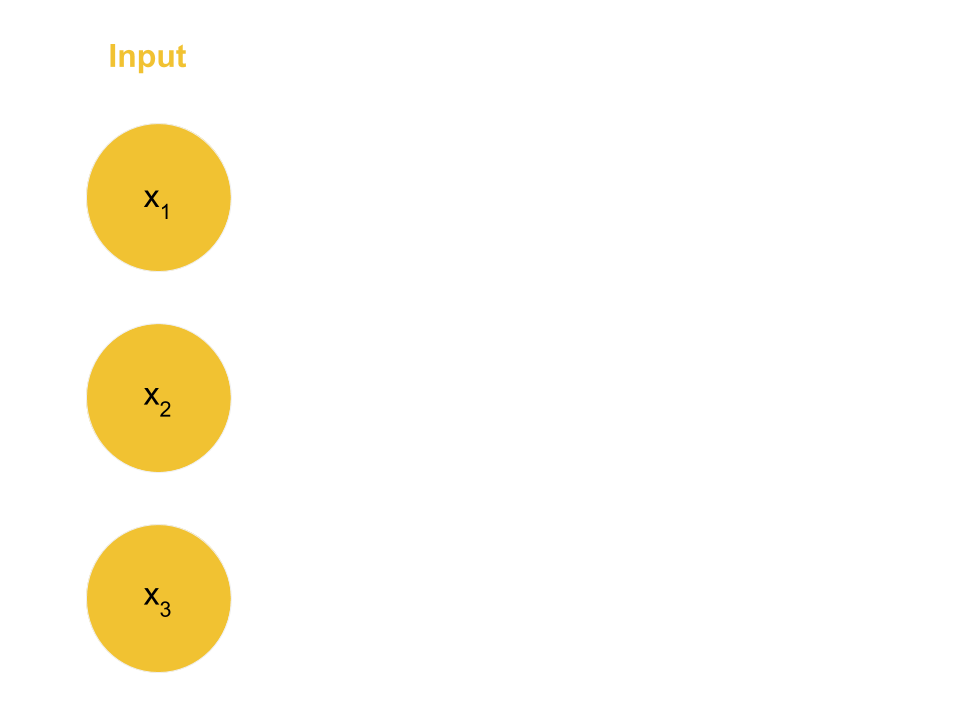
\includegraphics[width=6cm]{figure/neurep_one.png}
\end{figure}
\item In general, a $p$-dimensional input vector $\xv$ will be represented by $p$ nodes in the input layer.
\framebreak
%%%%%%%%%%%%%%%%%%%%%%%%%%%%%%%%%%%%%%%%%%%%%%%%%%%%%%%%%%%%%%%%%%

\item Next, weights $\mathbf{w}$ are represented by edges from the input layer.
\begin{figure}
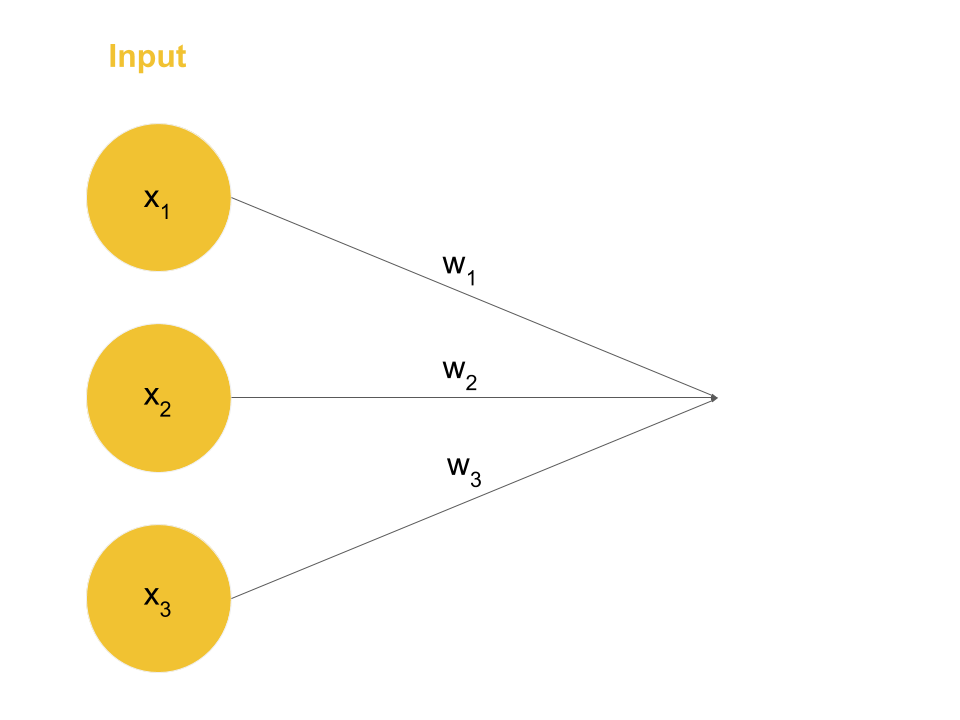
\includegraphics[width=6cm]{figure/neurep_two.png}
\end{figure}
\item The bias term $b$ is implicit here. It is often not visualized as a separate node.
\end{itemize}
\framebreak
%%%%%%%%%%%%%%%%%%%%%%%%%%%%%%%%%%%%%%%%%%%%%%%%%%%%%%%%%%%%%%%%%%

For an explicit graphical representation, we do a simple trick: 
\begin{itemize}
\item Add a constant feature to the inputs $\tilde{\xv} = (1, x_1, ..., x_p)^T$
\item and absorb the bias into the weight vector $\tilde{\bm{w}} = (b, w_1, ..., w_p)$.
\end{itemize}
The graphical representation is then: 
\begin{figure}
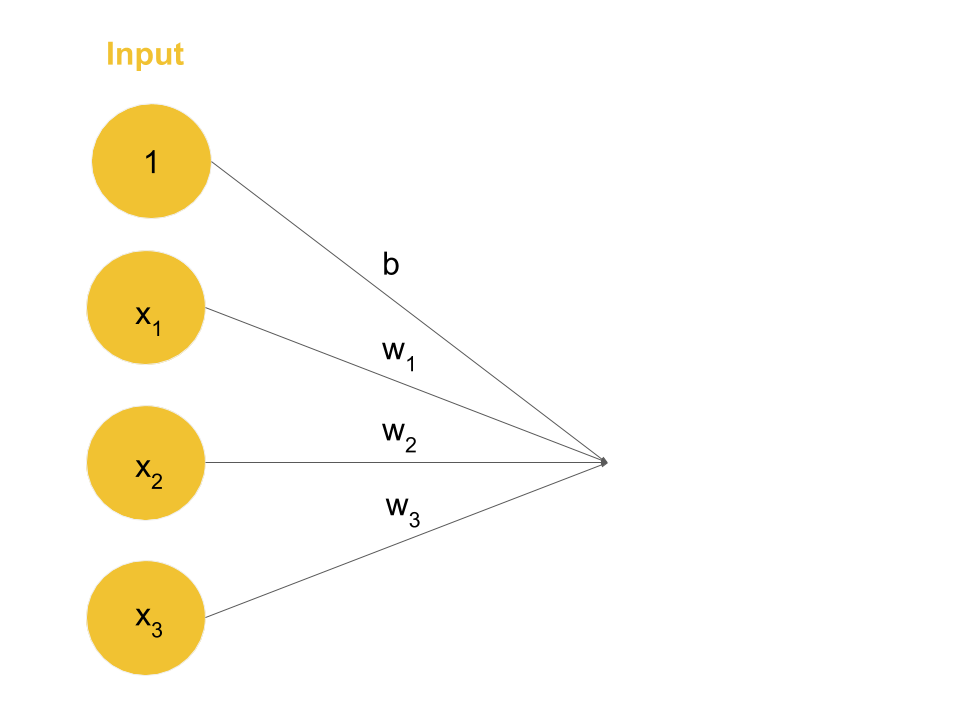
\includegraphics[width=7cm]{figure/neurep_bias.png}
\end{figure}
\framebreak
%%%%%%%%%%%%%%%%%%%%%%%%%%%%%%%%%%%%%%%%%%%%%%%%%%%%%%%%%%%%%%%%%%

\begin{itemize}
\item Finally, the computation $\tau(w_1x_1 + w_2x_2 + w_3x_3 + b)$ is represented by the neuron in the \enquote{output layer}.
\begin{figure}
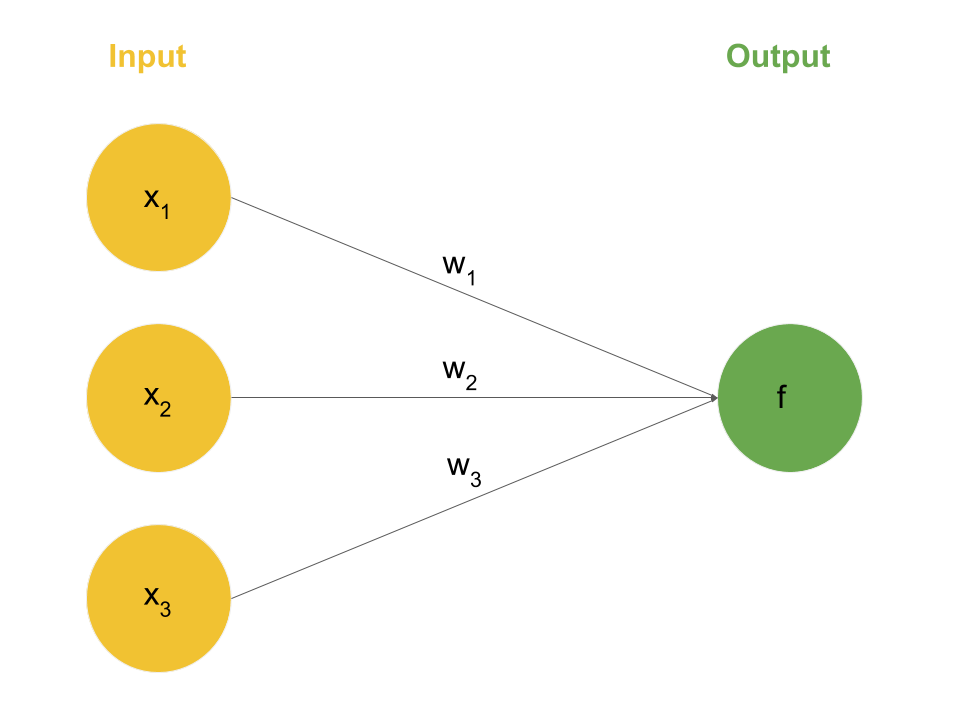
\includegraphics[width=6cm]{figure/neurep_three.png}
\end{figure}
\item Because this single neuron represents exactly the same hypothesis space as logistic regression, it can only learn linear decision boundaries.
\framebreak
%%%%%%%%%%%%%%%%%%%%%%%%%%%%%%%%%%%%%%%%%%%%%%%%%%%%%%%%%%%%%%%%%%

\item A nice thing about this graphical representation of functions is that you can picture the input vector being "fed" to the neuron on the left followed by a sequence of computations being performed from left to right. This is called a \textbf{forward pass}.
\end{itemize}
\vspace{1cm}
\begin{figure}
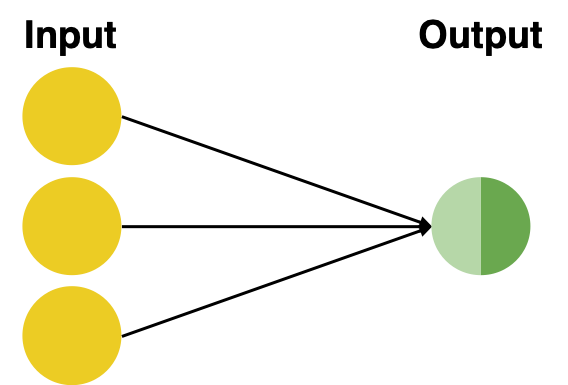
\includegraphics[width=5.5cm]{figure/forward_pass.png}
\end{figure}
\end{vbframe}
%%%%%%%%%%%%%%%%%%%%%%%%%%%%%%%%%%%%%%%%%%%%%%%%%%%%%%%%%%%%%%%%%%

\begin{frame} {A Single Neuron}
Therefore, a neuron performs a 2-step computation:
\begin{enumerate}
\item \textbf{Affine Transformation:} weighted sum of inputs plus bias.
\begin{figure}
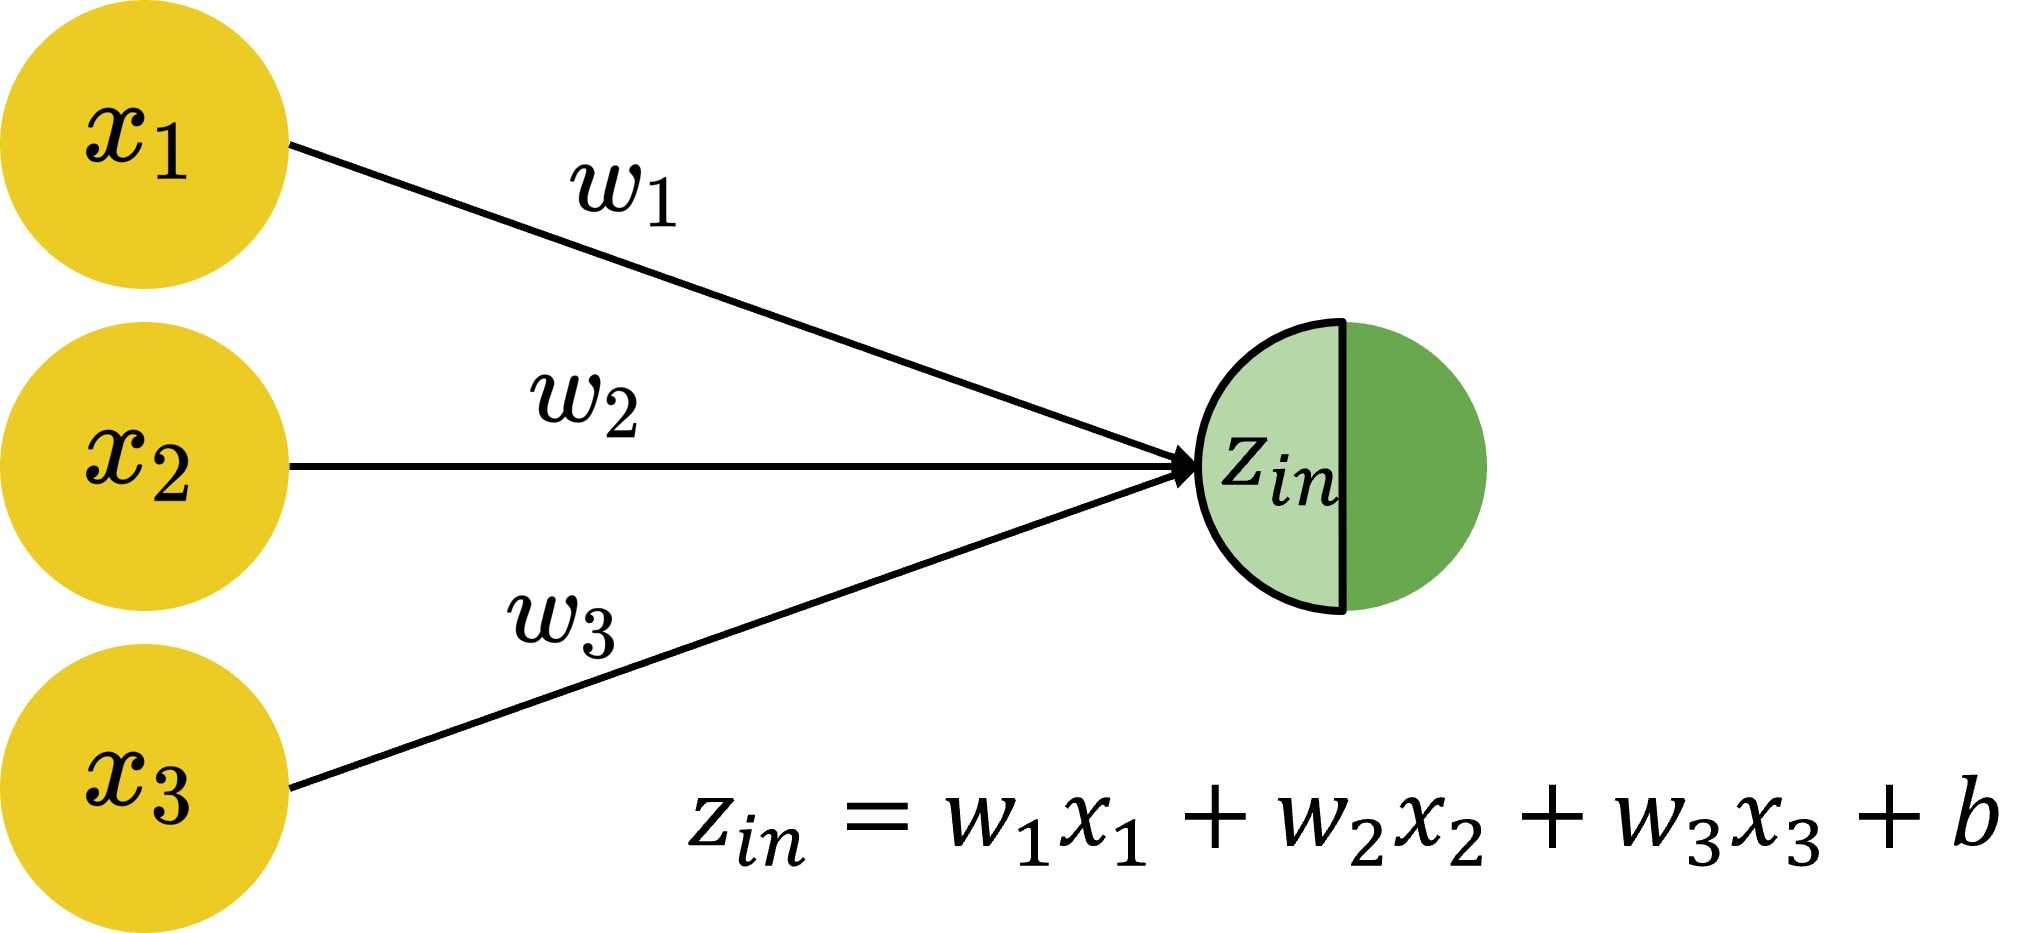
\includegraphics[width=5.5cm]{figure/step1-zin.jpg}
\end{figure}
\item \textbf{Non-linear Activation:} a non-linear transformation applied to the weighted sum.
\begin{figure}
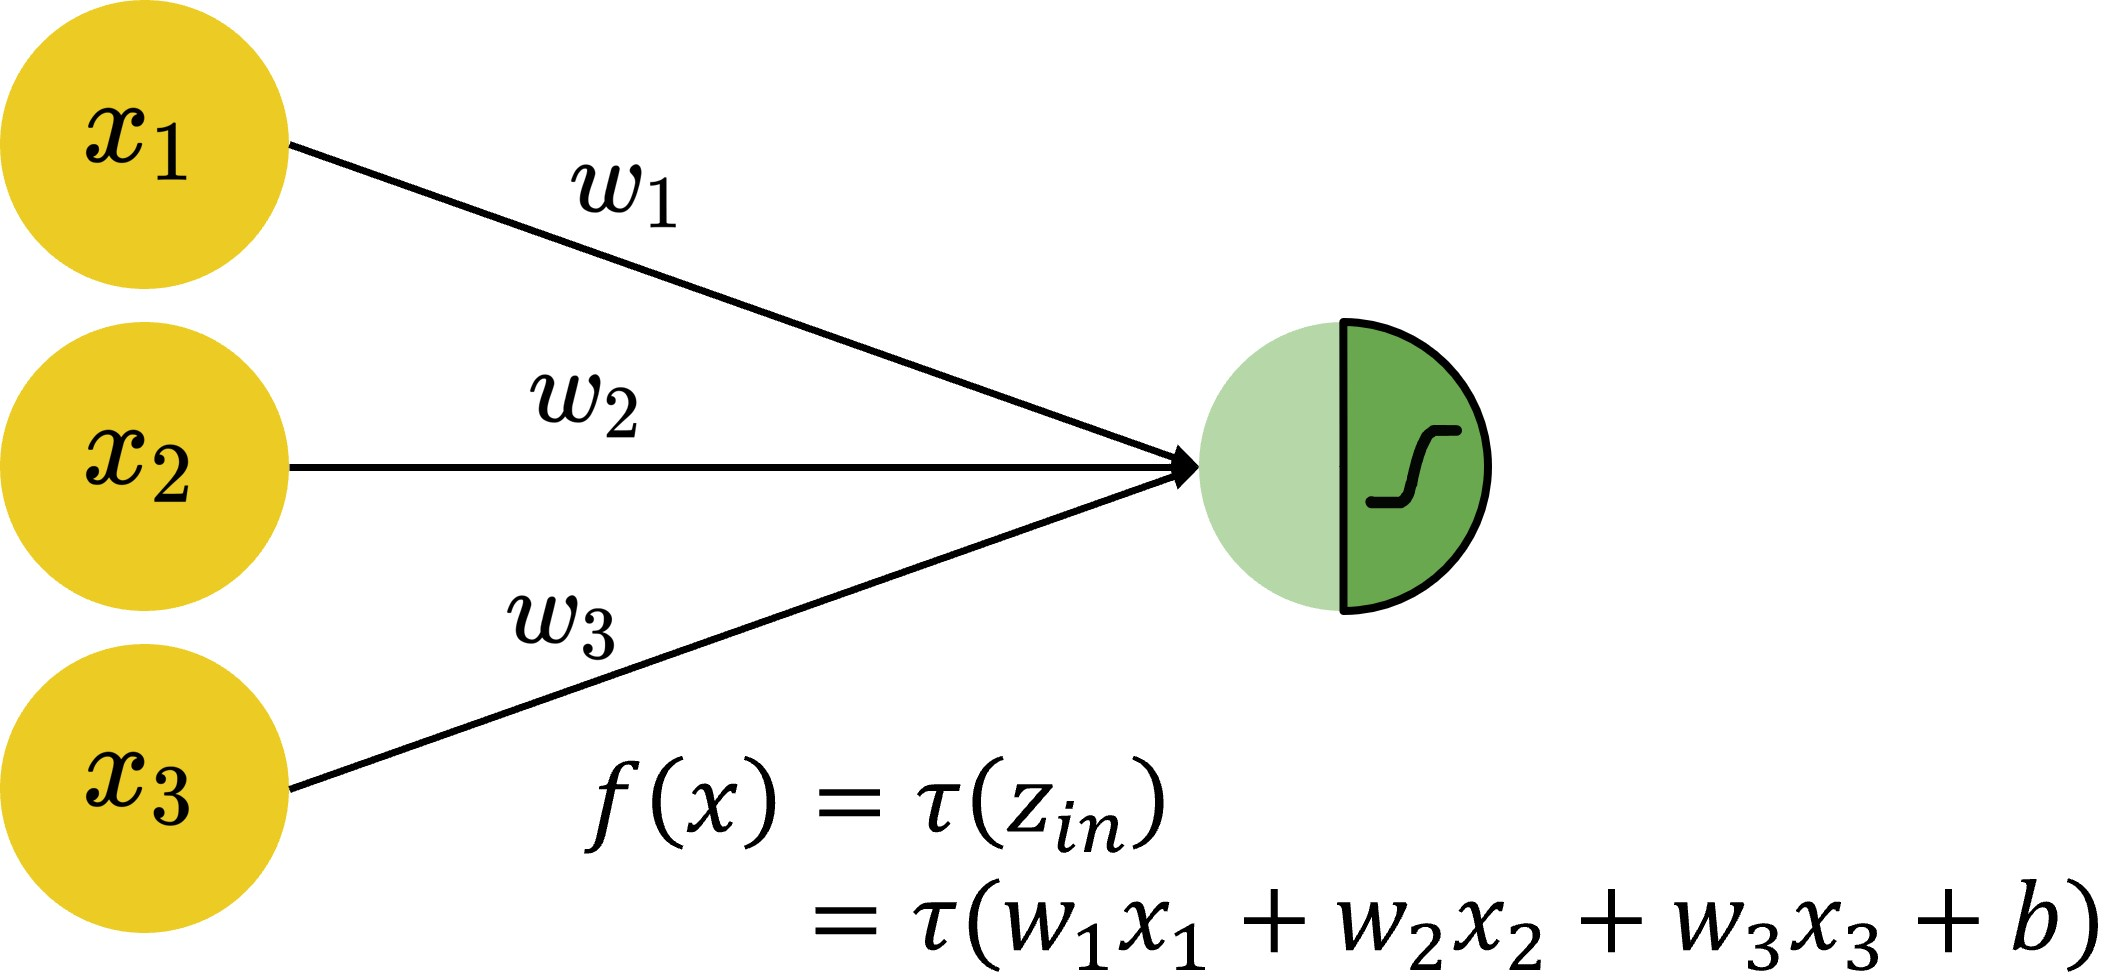
\includegraphics[width=5.5cm]{figure/step2-zin.jpg}
\end{figure}
\end{enumerate}
\end{frame}
%%%%%%%%%%%%%%%%%%%%%%%%%%%%%%%%%%%%%%%%%%%%%%%%%%%%%%%%%%%%%%%%%%

\begin{vbframe} {A Single Neuron}
\begin{itemize}
\item Even though all neurons compute a weighted sum in the first step, there is considerable flexibility in the type of activation function used in the second step.
\item For example, setting the activation function to logistic sigmoid function allows a neuron to represent logistic regression. The following neuron represents a logistic regression with two outputs.
\end{itemize}
\begin{figure}
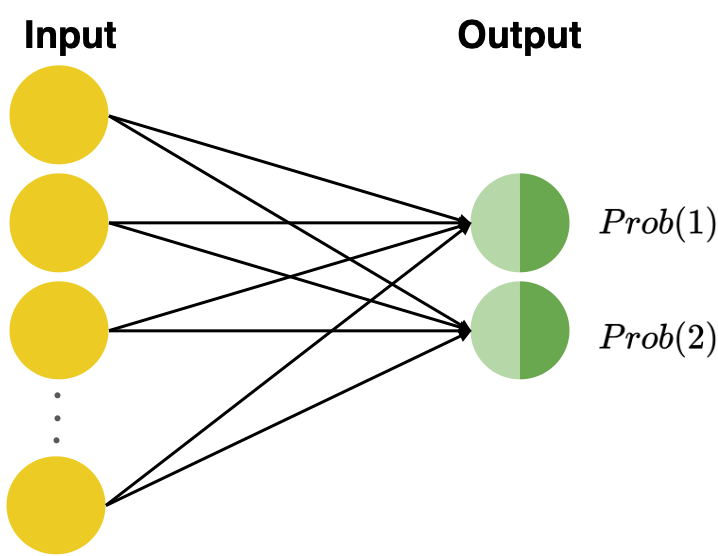
\includegraphics[width=5.5cm]{figure/logistic_regression.png}
\end{figure}
\end{vbframe}
%%%%%%%%%%%%%%%%%%%%%%%%%%%%%%%%%%%%%%%%%%%%%%%%%%%%%%%%%%%%%%%%%%

\begin{vbframe}{A Single Neuron}
\begin{itemize}
\item The hypothesis space that is formed by single neuron architectures is 
\begin{small}
$$\Hspace  = \left\{f: \R^p \to \R ~\bigg|~ \fx = \tau\left(\sum_{j = 1}^p w_j x_j + b\right), \wtw \in \R^p, b \in \R\right\}.$$ 
\end{small}
\item Both logistic regression and linear regression are subspaces of $\Hspace$ (if $\tau$ is the logistic sigmoid / identity function).  \end{itemize}
\vspace*{-0.48cm}
\begin{figure}
\centering
\scalebox{0.7}{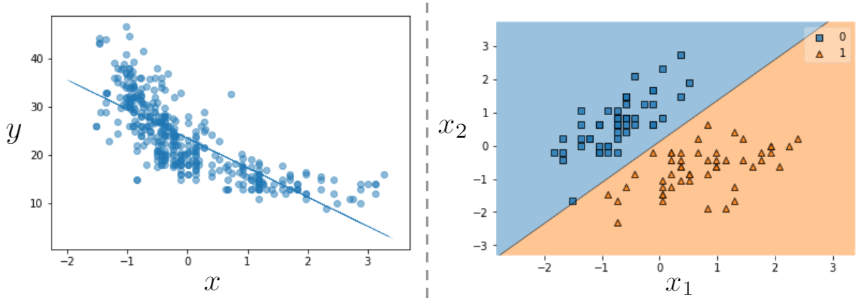
\includegraphics{figure/neuron_regcls.png}}
\vspace*{-0.2cm}
\begin{tiny}
\caption{\textit{Left}: A regression line learned by a single neuron. \textit{Right}: A decision-boundary learned by a single neuron in a binary classification task.}
\end{tiny}
\end{figure}
\end{vbframe}
%%%%%%%%%%%%%%%%%%%%%%%%%%%%%%%%%%%%%%%%%%%%%%%%%%%%%%%%%%%%%%%%%%

\begin{vbframe} {A Single Neuron: Optimization}
\begin{itemize}
\item To optimize this model, we minimize the empirical risk 
$$\riske = \frac{1}{n} \sumin \Lxyi,$$
where $\Lxy$ is a loss function. It compares the network's predictions $\fx$ to the ground truth $y$. 
\item For regression, we typically use the L2 loss (rarely L1): $$\Lxy = \frac{1}{2}(y - \fx)^2$$
\item For binary classification, we typically apply the cross entropy loss (also known as bernoulli loss): $$\Lxy = y \log \fx + (1 - y) \log(1 - \fx)$$
\framebreak 
%%%%%%%%%%%%%%%%%%%%%%%%%%%%%%%%%%%%%%%%%%%%%%%%%%%%%%%%%%%%%%%%%%

\vspace{.5cm}
\item For a single neuron, in both cases, the loss function is convex and the global optimum can be found with an iterative algorithm like gradient descent. 
\item In fact, a single neuron with logistic sigmoid function trained with the bernoulli loss does not only have the same hypothesis space as a logistic regression and is therefore the same model, but will also yield to the very same result when trained until convergence.
\item Note: In the case of regression and the L2-loss, the solution can
also be found analytically using the “normal equations”. However,
a closed-form solution is usually not available.
\end{itemize}
\end{vbframe} 
%%%%%%%%%%%%%%%%%%%%%%%%%%%%%%%%%%%%%%%%%%%%%%%%%%%%%%%%%%%%%%%%%%

\endlecture
\end{document}